\documentclass[ignorenonframetext,usenames,dvipsnames]{beamer}
\usepackage[spanish,english]{babel}
% or whatever

\usepackage{amsmath}
\usepackage{amsfonts}
\usepackage{amsthm}
\usepackage{mathtools}
\usepackage{cases}
\usepackage[utf8]{inputenc}
\usepackage{xmpmulti}
\usepackage{times}
\usepackage[T1]{fontenc}
\usepackage{color}
\usepackage{boxedminipage}
\usepackage[absolute,overlay]{textpos}
\usepackage{algorithm}
\usepackage{algpseudocode}
\usepackage{wasysym}
\usepackage{listings}
\usepackage{hyperref}
% Or whatever. Note that the encoding and the font should match. If T1
% does not look nice, try deleting the line with the fontenc.

\mode<article>
{
\usepackage{fullpage}
}

 \mode<presentation>
 {
  \usetheme{Boadilla}
  \setbeamertemplate{navigation symbols}{}
  \usefonttheme[onlymath]{serif}
  \setbeamertemplate{itemize items}[default]
  \setbeamertemplate{enumerate items}[default]
  %\setbeamertemplate{footline}[page number]{}
  \setbeamertemplate{footline}[frame number]{}
}

\newenvironment{reference}[2]{%
  \begin{textblock*}{\textwidth}(#1,#2)
    \tiny\it\color{red!50!black}}{\color{black}\end{textblock*}}

\newenvironment<>{varblock}[2][\textwidth]{
    \begin{center}
      \begin{minipage}{#1}
        \setlength{\textwidth}{#1}
          \begin{actionenv}#3
            \def\insertblocktitle{#2}
            \par
            \usebeamertemplate{block begin}}
  {\par
      \usebeamertemplate{block end}
    \end{actionenv}
  \end{minipage}
\end{center}}

%%%%%% Listings setup
\lstset{language=Python,
showstringspaces=false,
basicstyle=\tiny\ttfamily,
keywordstyle=\color{blue}\ttfamily,
stringstyle=\color{red}\ttfamily,
%commentstyle=\color{green}\ttfamily},
%backgroundcolor=\color{gray}
}

\DeclareMathOperator{\softmax}{softmax}

\title[] % (optional, use only with long paper titles)
{Modelos de toma de decisiones de humanos basado en aprendizaje reforzado}


\author[AJW]% (optional, use only with lots of authors)
{Alejandro Weinstein \\ alejandro.weinstein@uv.cl, @ajweinstein}
% - Use the \inst{?} command only if the authors have different
%   affiliation.

\institute[UV] % (optional, but mostly needed)
{Escuela de Ingeniería Biomédica \\
Universidad de Valparaíso}

\date {13 de diciembre de 2017}% (optional)

%\input{../macros.tex}
\graphicspath{{figures/}}
%\input{algs_defs.tex}

\begin{document}

\begin{frame}
    \titlepage
\end{frame}

%%%%%%%%%%%%%%%%%%%%%%%%%%%%%%%%%%%% Frame %%%%%%%%%%%%%%%%%%%%%%%%%%%%%%%%%%%%
\begin{frame}{Rescorla y Wagner:}
  \begin{quote}
    \begin{center}
    ``...organisms only learn when events violate their expectations.''
    \end{center}
  \end{quote}

  \begin{reference}{4mm}{90mm}
    R. A. Rescorla and A. R. Wagner, A theory of Pavlovian conditioning:
    Variations in the effectiveness of reinforcement and non reinforcement,
    Classical conditioning II: Current research and theory, vol. 2, pp. 64-99,
    1972.
  \end{reference}

\end{frame}

%%%%%%%%%%%%%%%%%%%%%%%%%%%%%%%%%%%% Frame %%%%%%%%%%%%%%%%%%%%%%%%%%%%%%%%%%%%
\begin{frame}{Condición experimental típica}

  \begin{itemize}
  \item El sujeto debe elegir entre un conjunto de opciones. Por ejemplo, debe
    presionar uno de los siguientes botones: \vspace{2ex}
  \begin{center}
    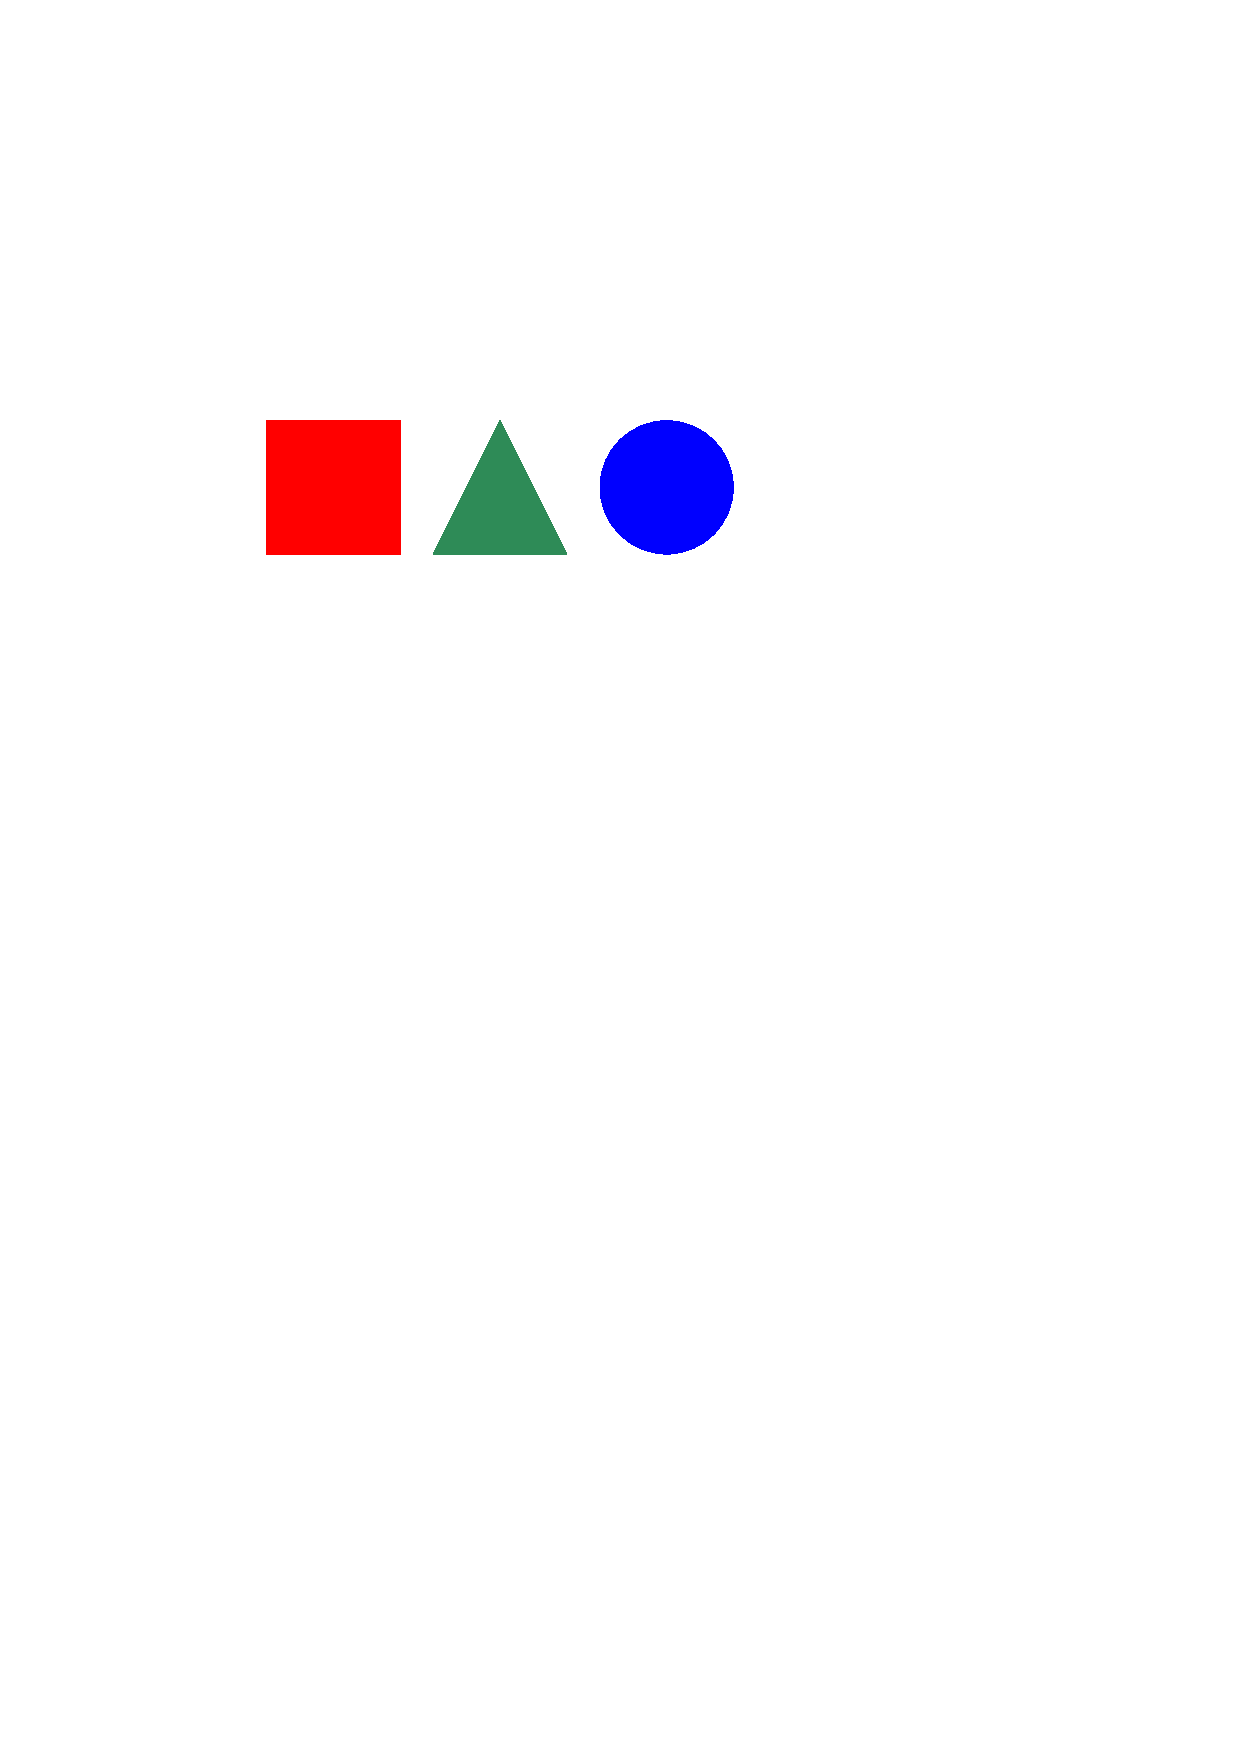
\includegraphics[scale=0.6]{exp}
  \end{center}
  \vspace{2ex}
  \item Según la opción elegida, recibe una recompensa.
  \item La secuencia se repite un número finito de veces.
  \item El objetivo es maximizar la recompensa total.
  \end{itemize}


  \vspace{2ex}
  \begin{center}
    Este problema también se conoce como \emph{Multi-armed bandit}
  \end{center}
\end{frame}

%%%%%%%%%%%%%%%%%%%%%%%%%%%%%%%%%%%% Frame %%%%%%%%%%%%%%%%%%%%%%%%%%%%%%%%%%%%
\begin{frame}{Condición experimental típica}

  En cada intento (trial) $t = 1, \ldots, T$, las recompensas se generan según
  las probabilidades:\footnote{Valores de ejemplo. Tanto los valores posibles
    que puede tener $r_t$, así como las probabilidades dependen de cada
    situación.}
  %
  \begin{gather*}
    P(r_t = 1 | a_t ={\color{red} \blacksquare} ) = 0.8 \\
    P(r_t = -1 | a_t ={\color{red} \blacksquare} ) = 0.2 \\
    P(r_t = 1 | a_t ={\color{OliveGreen}  \blacktriangle} ) = 0.5 \\
    P(r_t = -1 | a_t ={\color{OliveGreen} \blacktriangle} ) = 0.5 \\
    P(r_t = 1 | a_t ={\color{blue} \CIRCLE} ) = 0.2 \\
    P(r_t = -1 | a_t ={\color{blue} \CIRCLE} ) = 0.8 \\
  \end{gather*}

  Donde $T$ es el número de intentos disponibles, $a_t$ es la acción realizada en el trial $t$, y $r_t$ es la recompensa obtenida en el trial $t$.
\end{frame}

%%%%%%%%%%%%%%%%%%%%%%%%%%%%%%%%%%%% Frame %%%%%%%%%%%%%%%%%%%%%%%%%%%%%%%%%%%%
\begin{frame}{Condición experimental típica}
  \begin{block}{}
    \begin{center}
      ¡El sujeto no conoce estas probabilidades!
    \end{center}
  \end{block}
\end{frame}


%%%%%%%%%%%%%%%%%%%%%%%%%%%%%%%%%%%% Frame %%%%%%%%%%%%%%%%%%%%%%%%%%%%%%%%%%%%
\begin{frame}{Aprendizaje Reforzado (RL)}
  El problema se puede modelar como la interacción entre un \emph{agente} y el \emph{ambiente}:

  \begin{center}
    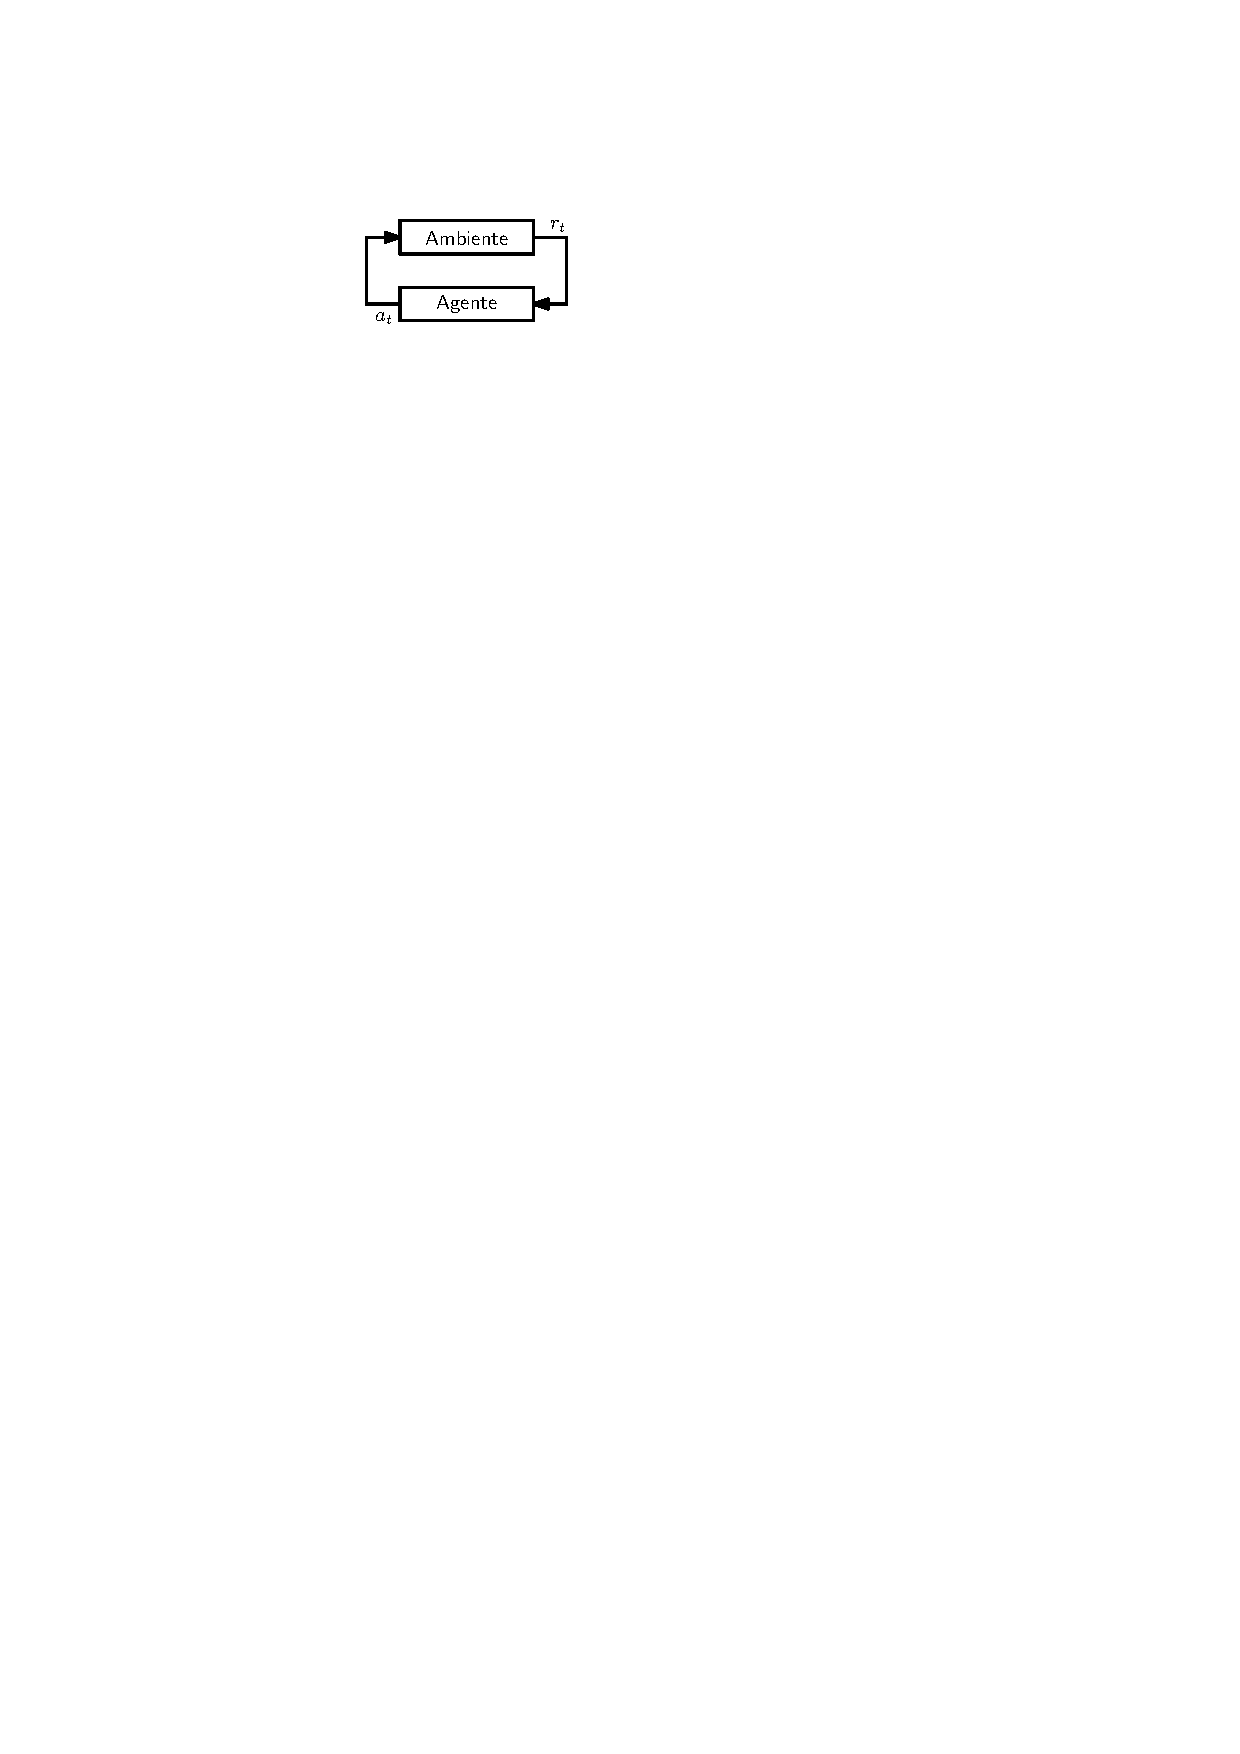
\includegraphics{rl}
  \end{center}

  El agente puede ser artificial o un ser vivo.
\end{frame}

%%%%%%%%%%%%%%%%%%%%%%%%%%%%%%%%%%%% Frame %%%%%%%%%%%%%%%%%%%%%%%%%%%%%%%%%%%%
\begin{frame}{Los dos problemas:}
  \begin{itemize}
  \item ¿Cómo modelamos el mecanismo utilizado por el agente para tomar las decisiones?
  \item Bajo la suposición de un modelo dado, y de las observaciones
    %
    \begin{equation*}
      (a_1, r_1), (a_2, r_2), \ldots (a_T, r_T)
    \end{equation*}
    %
    de las interacciones entre un agente y el ambiente, ¿cómo ajustamos los
    parámetros de dicho modelo?
  \end{itemize}
\end{frame}

%%%%%%%%%%%%%%%%%%%%%%%%%%%%%%%%%%%% Frame %%%%%%%%%%%%%%%%%%%%%%%%%%%%%%%%%%%%
\begin{frame}{¿Para qué?}
  \begin{itemize}
  \item Las diferencias entre los parámetros de distintos sujetos de una
    población, permite caracterizar a dichos sujetos.
  \item Correlacionar alguna variable del modelo con variables fisiológicas
    (EEG, fMRI, etc.) registradas en forma simultanea a la realización del
    experimento.
  \item Comparar distintos modelos.
  \end{itemize}
\end{frame}

%%%%%%%%%%%%%%%%%%%%%%%%%%%%%%%%%%%% Frame %%%%%%%%%%%%%%%%%%%%%%%%%%%%%%%%%%%%
\begin{frame}{El modelo ``action-value''}

\textbf{Objetivo:} Elegir secuencia de acciones de tal forma de que se maximice la recompensa total
%
\begin{equation*}
  R = \sum_{t=1}^T r_t.
\end{equation*}

  \begin{reference}{4mm}{91mm}
    Sutton, Richard S., and Andrew G. Barto. Reinforcement learning: An
    introduction. Vol. 1. No. 1. Cambridge: MIT press, \textbf{Second Edition}, 2017.
    (\url{http://incompleteideas.net/book/the-book-2nd.html})
  \end{reference}
\end{frame}

%%%%%%%%%%%%%%%%%%%%%%%%%%%%%%%%%%%% Frame %%%%%%%%%%%%%%%%%%%%%%%%%%%%%%%%%%%%
\begin{frame}{El modelo ``action-value''}
En cada iteración el agente actualiza el \emph{action-value} según la regla
%
\begin{equation*}
  Q_{t+1}(a_t) = Q_t(a_t) + \alpha (r_t - Q_t(a_t))
\end{equation*}
%
y selecciona una acción en forma estocástica usando la regla \emph{softmax} que
asigna probabilidades a cada acción según
\begin{equation*}
  P(a_t = a_j) = \frac{e^{\beta Q_t(a)}}{\sum_{i=1}^{|\mathcal{A}|} e^{\beta Q_t(a_i)}},
  \quad j \in \mathcal{A},
\end{equation*}
%
donde los parámetros del modelo son la tasa de aprendizaje (\emph{learning
  rate}) $\alpha$ y la temperatura inversa $\beta$, y $\mathcal{A}$ es el
conjunto de posibles acciones.
\end{frame}


%%%%%%%%%%%%%%%%%%%%%%%%%%%%%%%%%%%% Frame %%%%%%%%%%%%%%%%%%%%%%%%%%%%%%%%%%%%
\begin{frame}{El modelo ``action-value''}

  Es útil pensar en $Q_t$ como en una tabla que se actualiza en la medida que
  se interactúa con el ambiente. Por ejemplo:
  %
  \begin{center}
    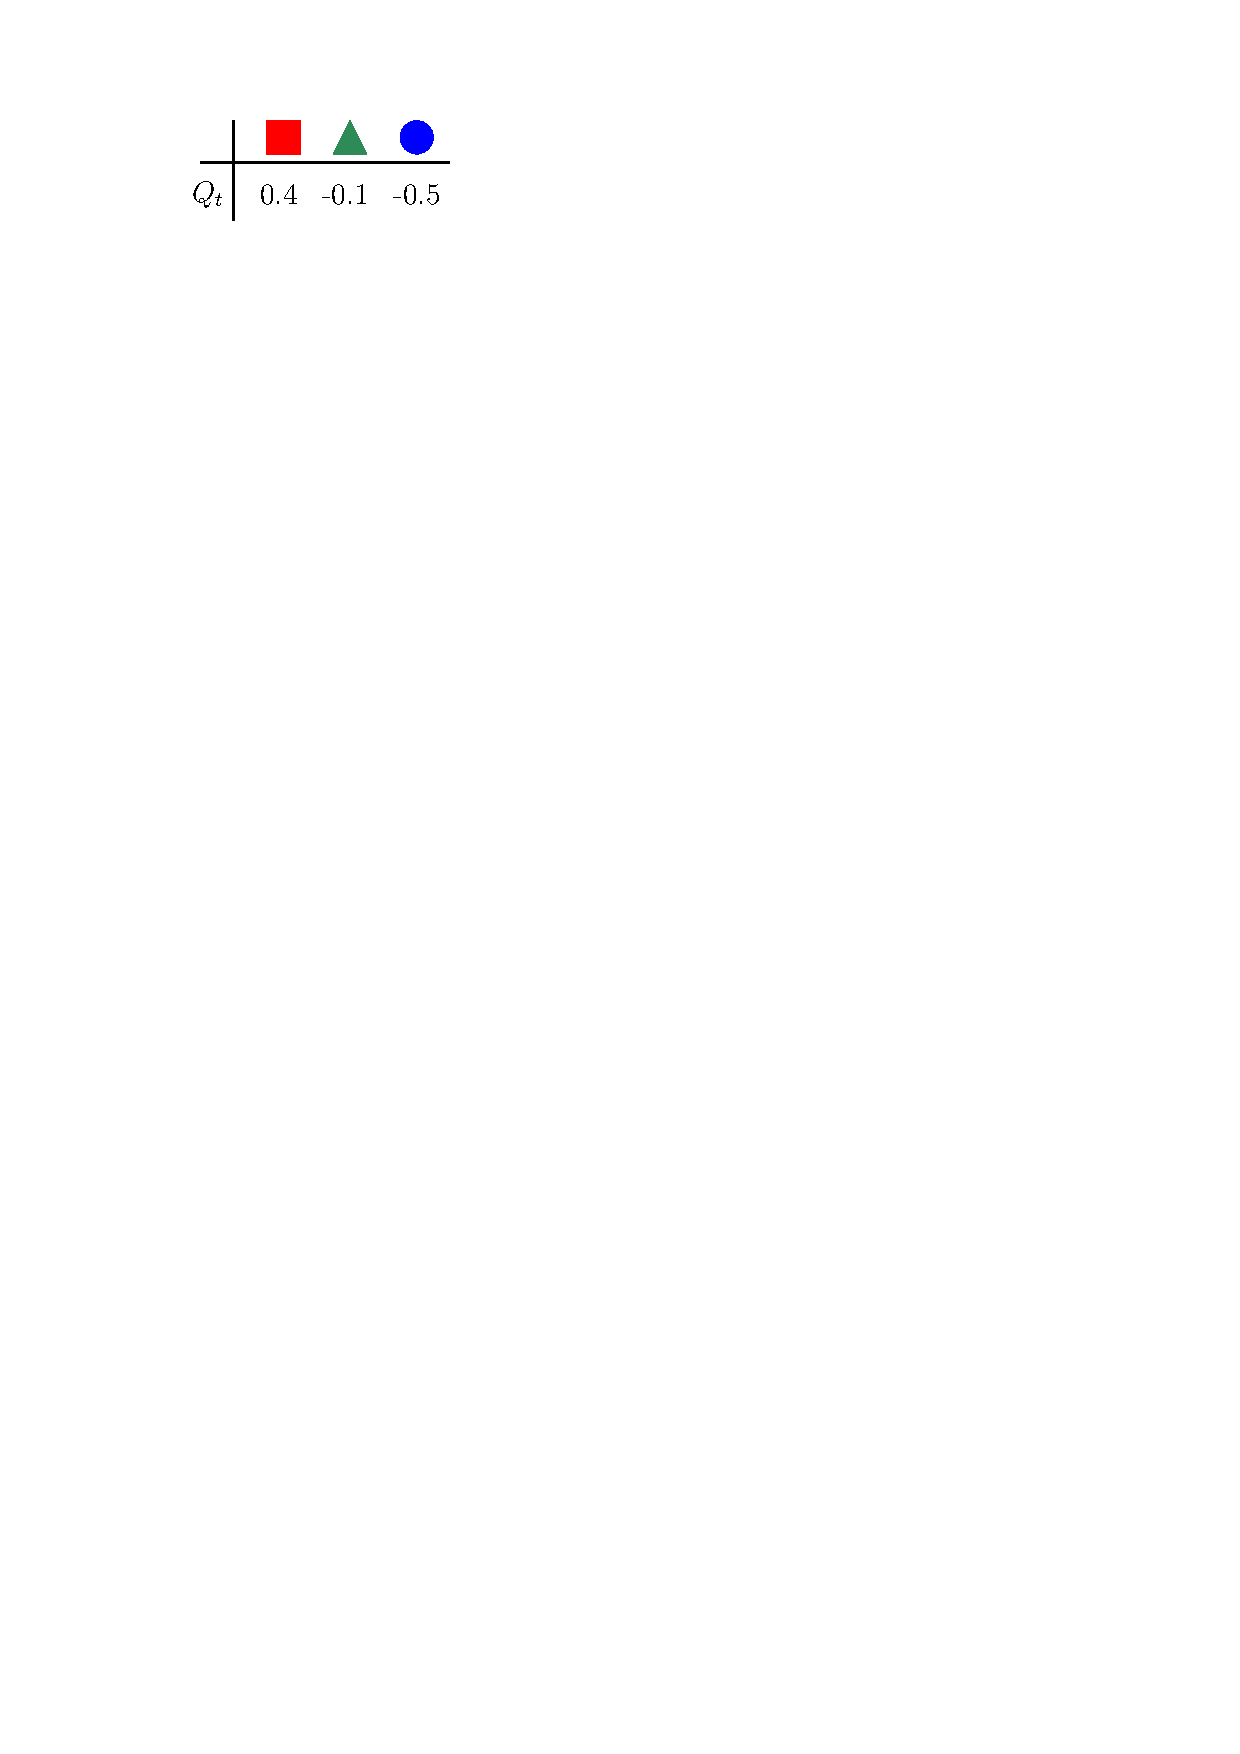
\includegraphics[page=1,scale=0.8]{Q}
    %
    \begin{gather*}
      a_t = {\color{OliveGreen}  \blacktriangle}, r_t=1, \alpha=0.2 \\
      -0.1 + 0.2(-0.1 + 1) = 0.08 \\
      \downarrow
    \end{gather*}
    %
    \includegraphics[page=2,,scale=0.8]{Q}

  \end{center}

  \begin{block}{}
    \begin{center}
      $Q$ es una estimación del valor esperado de cada acción
    \end{center}

    \end{block}

\end{frame}


%%%%%%%%%%%%%%%%%%%%%%%%%%%%%%%%%%%% Frame %%%%%%%%%%%%%%%%%%%%%%%%%%%%%%%%%%%%
\begin{frame}{El modelo ``action-value''}



\begin{equation*}
  Q_{t+1}(a_t) = Q_t(a_t) + \alpha (\underbrace{r_t - Q_t(a_t)}_{\text{?}})
\end{equation*}
\pause
\begin{equation*}
  Q_{t+1}(a_t) = Q_t(a_t) + \alpha (\underbrace{r_t - Q_t(a_t)}_{\text{Señal de error}})
\end{equation*}

En la literatura, a esta señal de error se le conoce como ``Temporal Difference''.
\vspace{2ex}

\pause
Rescorla y Wagner:
  \begin{quote}
    \begin{center}
    ``...organisms only learn when events violate their expectations.''
    \end{center}
  \end{quote}

\end{frame}

%%%%%%%%%%%%%%%%%%%%%%%%%%%%%%%%%%%% Frame %%%%%%%%%%%%%%%%%%%%%%%%%%%%%%%%%%%%
\begin{frame}{Sobre softmax}
  Para todos los casos, $Q({\color{red} \blacksquare}) = 5, Q({\color{OliveGreen}  \blacktriangle}) = 5.5, Q({\color{blue} \CIRCLE}) = 4.5$
  \begin{center}
    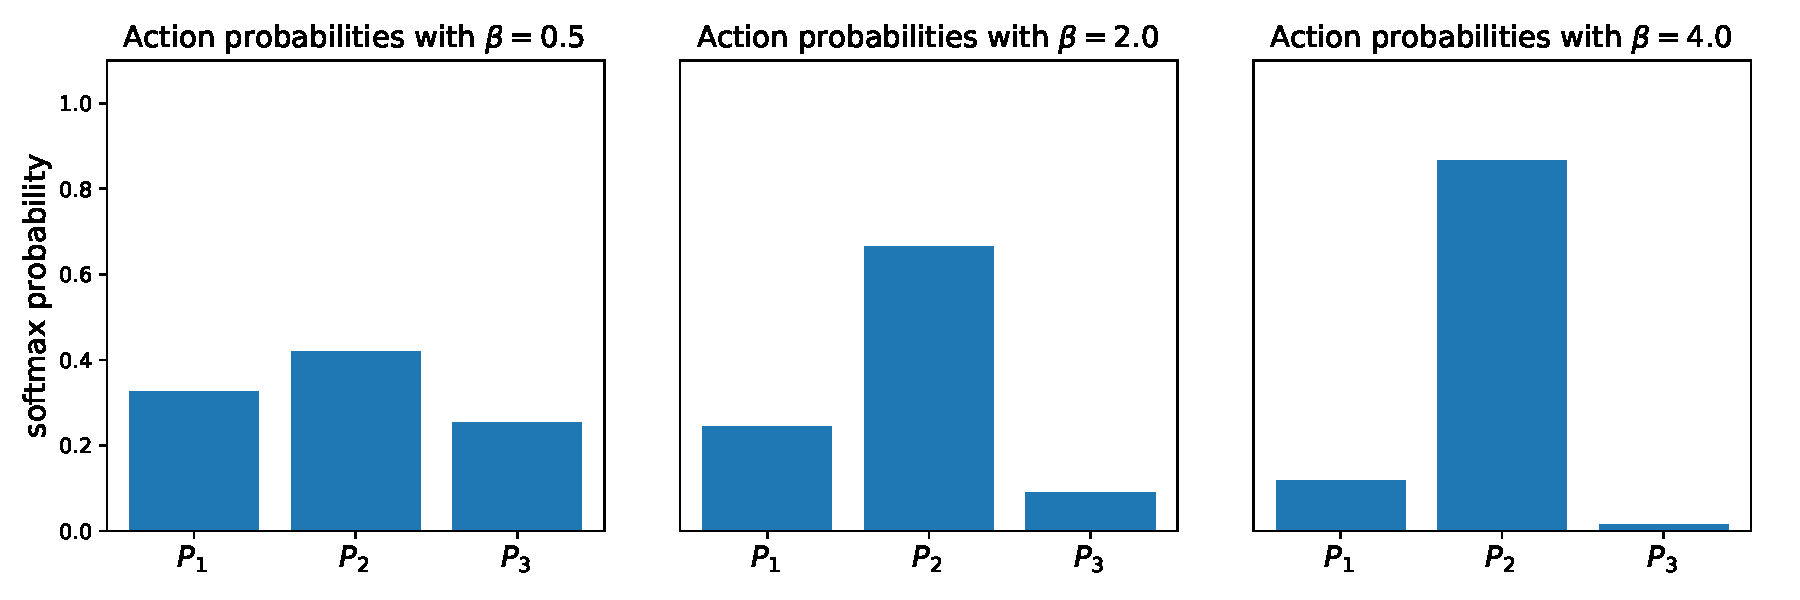
\includegraphics[width=0.9\columnwidth]{softmax}
  \end{center}

  En general,

  \begin{equation*}
    \lim_{\beta \to 0 } \frac{e^{\beta x_j}}{\sum e^{\beta x_i}} = \frac{1}{|\mathcal{A}|}
  \end{equation*}
    \begin{equation*}
      \lim_{\beta \to \infty } \frac{e^{\beta x_j}}{\sum e^{\beta x_i}} =
      \begin{cases}
        1 &\text{ si } x_j > x_i\\
        0 &\text{ si } x_j < x_i \\
      \end{cases}
      \qquad j \neq i.
  \end{equation*}


  Notebook demo...
\end{frame}

%%%%%%%%%%%%%%%%%%%%%%%%%%%%%%%%%%%% Frame %%%%%%%%%%%%%%%%%%%%%%%%%%%%%%%%%%%%
\begin{frame}[fragile]{Implementando el modelo ``action-value''}

  \begin{columns}
    \begin{column}{0.4\linewidth}
\begin{lstlisting}
class Environment(object):
    def __init__(self):
        self.actions = ('square',
                        'triangle',
                        'circle')
        self.prob_win = {'square': 0.8,
                         'triangle': 0.5,
                         'circle': 0.2}
        self.n = len(self.actions)

    def reward(self, action):
        p = self.prob_win[action]
        if np.random.rand() < p:
            r = 1
        else:
            r = -1
        return r
\end{lstlisting}

    \end{column}
    \begin{column}{0.6\linewidth}
\begin{lstlisting}
  class Agent(object):
    def __init__(self, environment, alpha, beta):
        # ...
    def run(self):
        action = self.choose_action()
        action_l = self.actions[action])
        reward = self.environment.reward(action_l)
        self.update_action_value(action, reward)

    def choose_action(self):
        p = softmax(self.Q, self.beta)
        actions = range(self.n)
        action = np.random.choice(actions, p=p)
        return action

    def update_action_value(self, action, reward):
        error = reward - self.Q[action]
        self.Q[action] += self.alpha * error
\end{lstlisting}
    \end{column}
  \end{columns}

  \begin{center}
    \begin{tabular}{c}
  \begin{lstlisting}
    if __name__ == '__main__':
        env = Environment()
        agent = Agent(env, 0.1, 1.2)
        T = 100
        for _ in range(T):
            agent.run()
  \end{lstlisting}
  \end{tabular}
  \end{center}

\end{frame}

%%%%%%%%%%%%%%%%%%%%%%%%%%%%%%%%%%%% Frame %%%%%%%%%%%%%%%%%%%%%%%%%%%%%%%%%%%%
\begin{frame}{Implementando el modelo ``action-value''}
  \begin{center}
    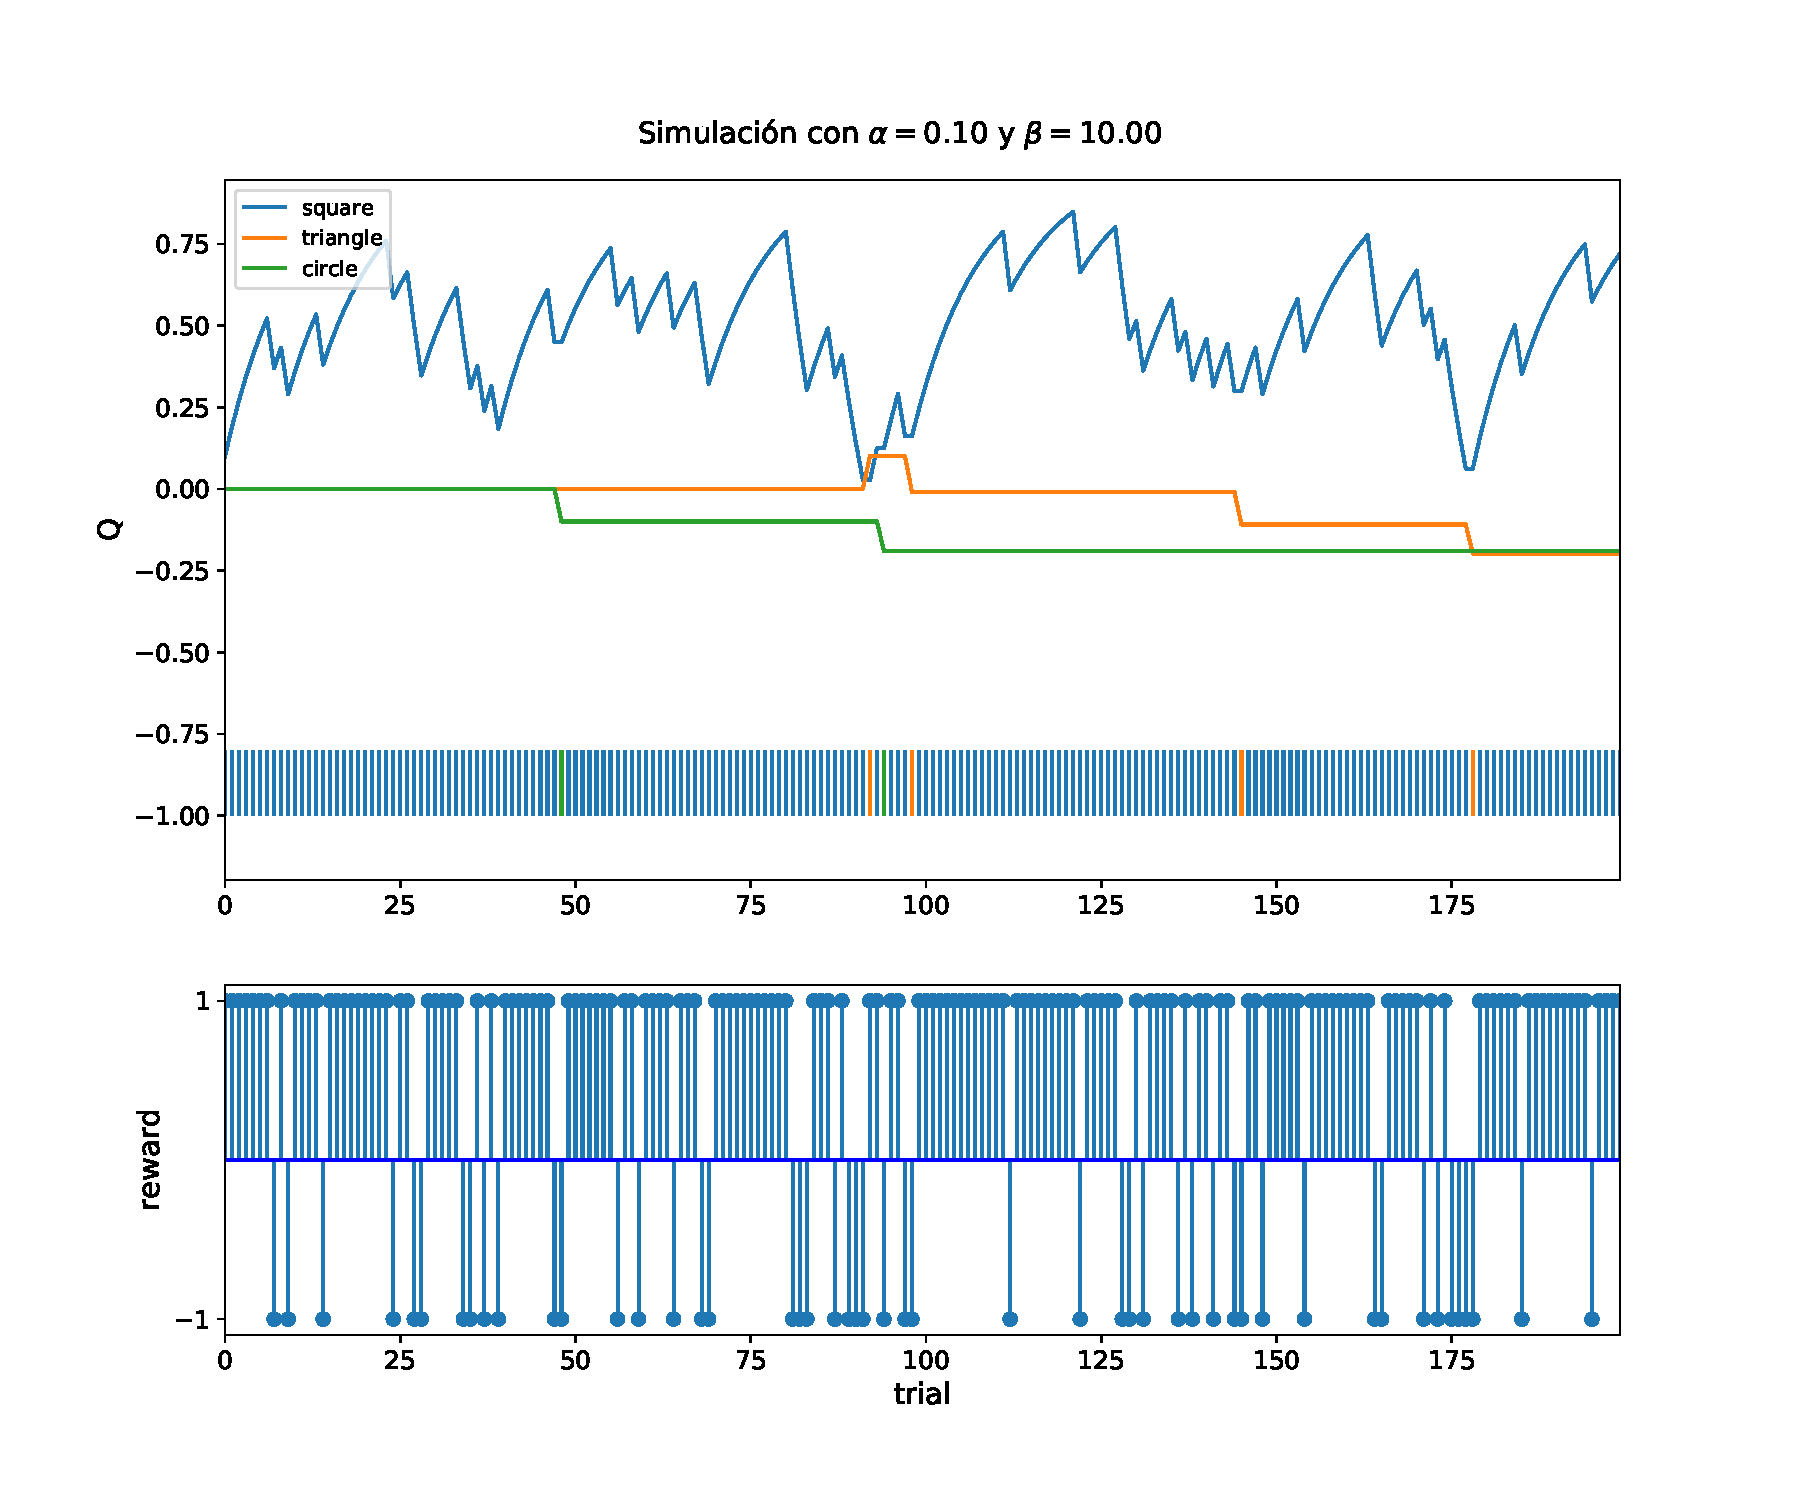
\includegraphics[scale=0.35]{action_value_sim}
  \end{center}
\end{frame}
%%%%%%%%%%%%%%%%%%%%%%%%%%%%%%%%%%%% Frame %%%%%%%%%%%%%%%%%%%%%%%%%%%%%%%%%%%%
\begin{frame}{Estimación de los parámetros del modelo}

\textbf{Problema:} A partir de la secuencia de pares acción-recompensa
%
\begin{equation*}
(a_1, r_1), (a_2, r_2), \ldots (a_T, r_T)
\end{equation*}
%
observados durante la interacción de un agente con un ambiente dado, estimar los parámetros del modelo que se asume utiliza dicho agente. Por ejemplo, estimar $\alpha$ y $\beta$ del modelo ``action-value''.


  \begin{reference}{4mm}{91mm}
    Daw, Nathaniel D. ``Trial-by-trial data analysis using computational
    models.'' Decision making, affect, and learning: Attention and performance
    XXIII 23 (2011): 3-38.
  \end{reference}

\end{frame}

%%%%%%%%%%%%%%%%%%%%%%%%%%%%%%%%%%%% Frame %%%%%%%%%%%%%%%%%%%%%%%%%%%%%%%%%%%%
\begin{frame}{Estimación de los parámetros del modelo}

  Los parámetros del modelo se obtienen utilizando el principio de máxima
  verosimilitud (máximum likelihood). La verosimilitud de los parámetros está
  dada por
  %
  \begin{equation*}
    \mathcal{L}(\alpha, \beta) = \prod_{t=1}^T P(a_t, c_t).
  \end{equation*}
  %
  Si asumimos el modelo ``action-value'', la probabilidad $P(a_t, c_t)$ se
  calcula usando las reglas de actualización del action-value y de softmax. Luego,
  %
  \begin{equation*}
     \widehat{\alpha}, \widehat{\beta} =
     \underset{0\leq\alpha \leq 1, 0 \leq \beta}{\operatorname{argmin}}     -\log(\mathcal{L}(\alpha, \beta)).
  \end{equation*}

  En la práctica es conveniente asignar un límite superior a $\beta$, por
  ejemplo, $0 \leq \beta \leq 2$.
\end{frame}

%%%%%%%%%%%%%%%%%%%%%%%%%%%%%%%%%%%% Frame %%%%%%%%%%%%%%%%%%%%%%%%%%%%%%%%%%%%
\begin{frame}{Cálculo de la función de verosimilitud}

Supongamos que observamos la secuencia
%
$
({\color{OliveGreen}  \blacktriangle}, 1),
({\color{blue} \CIRCLE}, -1)
({\color{blue} \CIRCLE}, -1)
$. La función $Q_t$ evoluciona como (asumiendo valor inicial 0):
%
\begin{gather*}
  Q_1({\color{OliveGreen}  \blacktriangle}) = 0 + \alpha(1-0) = \alpha \\
  Q_2({\color{blue} \CIRCLE}) = 0 + \alpha(-1-0) = -\alpha \\
  Q_3({\color{blue} \CIRCLE}) = -\alpha + \alpha(-1-(-\alpha)) =
  -2\alpha + \alpha^2.
\end{gather*}
%
Y la función de verosimilitud es
%
\begin{align*}
  \mathcal{L}(\alpha, \beta)  = &\softmax({\color{OliveGreen}  \blacktriangle}, (0,0,0), \beta) \cdot \\
  &\softmax({\color{blue} \CIRCLE}, (\alpha, 0, 0), \beta) \cdot \\
  &\softmax({\color{blue} \CIRCLE}, (\alpha, 0, -\alpha), \beta).
\end{align*}
\end{frame}

%%%%%%%%%%%%%%%%%%%%%%%%%%%%%%%%%%%% Frame %%%%%%%%%%%%%%%%%%%%%%%%%%%%%%%%%%%%
\begin{frame}{Ejemplo de función de verosimilitud}

  \begin{center}
    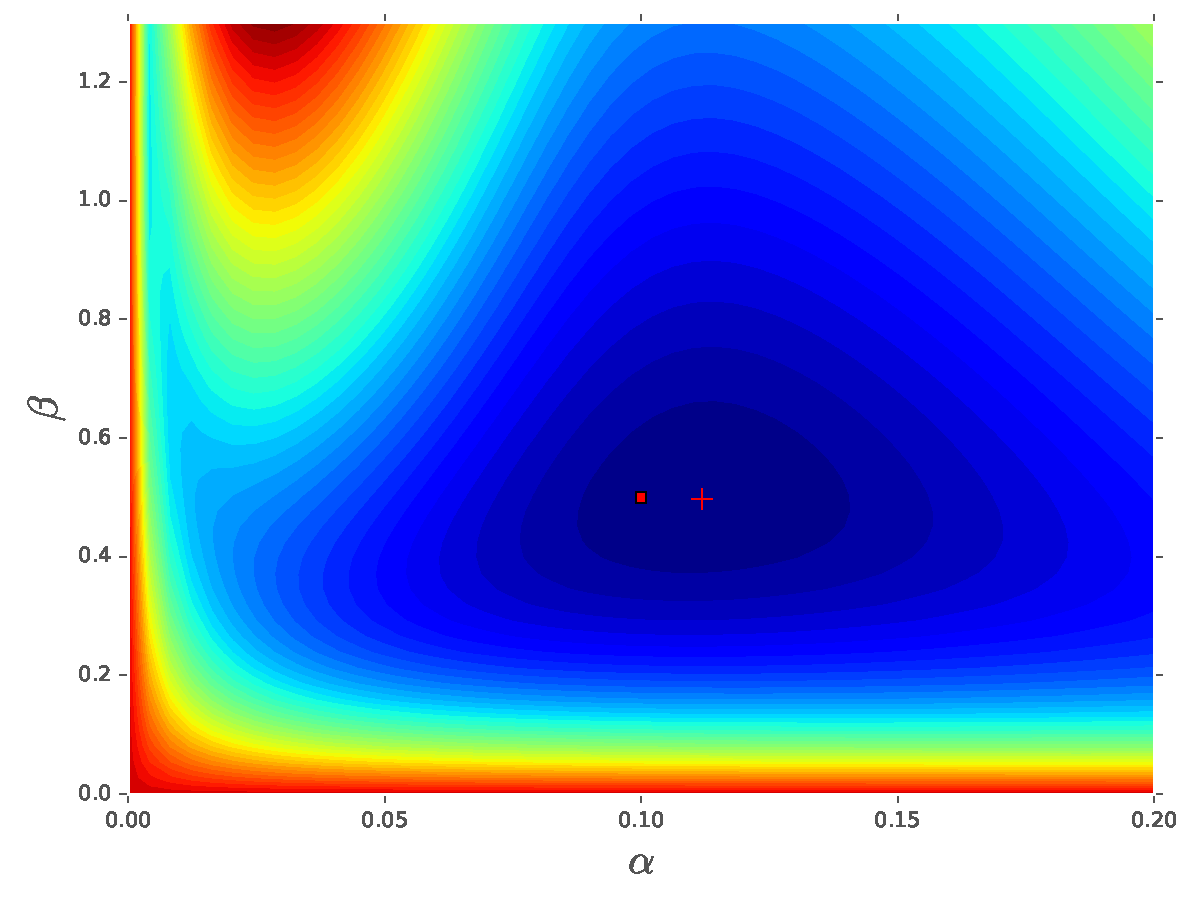
\includegraphics[width=0.7\columnwidth]{likelihood}
  \end{center}

  Los datos corresponden a un agente (artificial) operando con $\alpha=0.1$ y
  $\beta=0.5$ (cuadrado rojo). Los parámetros estimados utilizando el principio
  de máxima verosimilitud son $\widehat{\alpha}=0.11$ y $\widehat{\beta}=0.49$
  (cruz roja).
\end{frame}


%%%%%%%%%%%%%%%%%%%%%%%%%%%%%%%%%%%% Frame %%%%%%%%%%%%%%%%%%%%%%%%%%%%%%%%%%%%
\begin{frame}[fragile]{Implementando estimación de parámetros usando ML}


\begin{lstlisting}
class ML(object):
    def __init__(self, log):
        self.rewards = log['reward']
        label_to_n = {'square': 0, 'triangle': 1, 'circle': 2}
        self.actions = [label_to_n[a] for a in log['action']]
        self.n_actions = 3

    def neg_log_likelihood(self, alphabeta):
        alpha, beta = alphabeta
        prob_log = 0
        Q = np.zeros(self.n_actions)
        for action, reward in zip(self.actions, self.rewards):
            Q[action] += alpha * (reward - Q[action])
            prob_log += np.log(softmax(Q, beta)[action])

        return -prob_log

    def fit(self):
        bounds = ((0, 1), (0, 2))
        r = minimize(self.neg_log_likelihood, [0.1, 0.1],
                     method='L-BFGS-B',
                     bounds=bounds)
        return r
\end{lstlisting}

\end{frame}

%%%%%%%%%%%%%%%%%%%%%%%%%%%%%%%%%%%% Frame %%%%%%%%%%%%%%%%%%%%%%%%%%%%%%%%%%%%
\begin{frame}{Referencias anotadas}
  \begin{itemize}
  \item Sutton, Richard S., and Andrew G. Barto. Reinforcement learning: An
    introduction. Vol. 1. No. 1. Cambridge: MIT press, Second Edition, 2017 (\url{http://incompleteideas.net/book/the-book-2nd.html}).

    \begin{quote}
      Ver capítulo 2 para más detalles sobre el modelo ``action-value'', y
      capítulos 14 y 15 para relación entre RL con psicología y neurociencia.
    \end{quote}

  \item  Daw, Nathaniel D. ``Trial-by-trial data analysis using computational
    models.'' Decision making, affect, and learning: Attention and performance
    XXIII 23 (2011): 3-38.

    \begin{quote}
      Todos los detalles de estimación de parámetros RL usando ML, incluyendo
      incerteza en los parámetros, y comparación de modelos.
    \end{quote}
\end{itemize}
\end{frame}

%%%%%%%%%%%%%%%%%%%%%%%%%%%%%%%%%%%% Frame %%%%%%%%%%%%%%%%%%%%%%%%%%%%%%%%%%%%
\begin{frame}{Referencias anotadas}
  \begin{itemize}
  \item Dayan, Peter, and Laurence F. Abbott. Theoretical neuroscience. Vol. 806. Cambridge, MA: MIT Press, 2001.

    \begin{quote}
      Ver capítulo 9 para más detalles sobre el desarrollo del modelo
      ``action-value'', partiendo desde el condicionamiento clásico.
    \end{quote}

  \item Littman, Michael L. ``Reinforcement learning improves behaviour from evaluative feedback.'' Nature 521.7553 (2015): 445-451.

    \begin{quote}
      Revisión general de RL, con mención sobre el uso de RL como modelo de
      aprendizaje animal.
    \end{quote}

  \item Wiering, Marco, and Martijn van Otterlo, eds. Reinforcement Learning: State-of-the-Art. Vol. 12. Springer Science \& Business Media, 2012.

    \begin{quote}
      Ver capítulo 16 para más información sobre la relación entre RL y
      cognición, incluyendo rol de la dopamina y ganglio basal.
    \end{quote}

\end{itemize}
\end{frame}

%%%%%%%%%%%%%%%%%%%%%%%%%%%%%%%%%%%% Frame %%%%%%%%%%%%%%%%%%%%%%%%%%%%%%%%%%%%
\begin{frame}{Referencias anotadas}
  \begin{itemize}
\item FitzGerald, Thomas HB, Raymond J. Dolan, and Karl Friston. ``Dopamine, reward learning, and active inference.'' Frontiers in computational neuroscience 9 (2015).

  \begin{quote}
    Modelo alternativo de aprendizaje, basado en energía libre.
  \end{quote}

\end{itemize}
\end{frame}
\end{document}

%%% Local Variables:
%%% mode: latex
%%% TeX-master: t
%%% Local IspellDict: castellano
%%% End:

%%%
